\documentclass[11pt,a4paper]{article}

\usepackage[margin=2.5cm]{geometry}
\usepackage[T1]{fontenc}
\usepackage{lmodern}
\usepackage{microtype}
\usepackage{booktabs}
\usepackage{tabularx}
\usepackage{xcolor}
\usepackage{listings}
\usepackage{tikz}
\usetikzlibrary{arrows.meta,positioning,fit,backgrounds}
\usepackage[hidelinks]{hyperref}

\emergencystretch=3em
\newcolumntype{Y}{>{\raggedright\arraybackslash}X}
\lstset{basicstyle=\ttfamily\small, columns=fullflexible, frame=single, breaklines=true}
\newcommand{\file}[1]{\nolinkurl{#1}}
\newcommand{\test}[1]{\nolinkurl{#1}}
\def\UrlBreaks{\do\_\do/\do.\do-}
\newcommand{\commit}[1]{\texttt{#1}}

\title{Cleaning Manager: Authorization Across Component Boundaries\\[4pt]
\large Software Security, Assignment I}
\author{Marcus Mitelea, 202511022\\Aarhus University}
\date{October 2026}

\begin{document}
\maketitle

\noindent Repository: \url{https://github.com/mitmarcus/AU_SoftSec}, folder \file{Assignment_1}. All paths below are relative to that folder, and line numbers refer to tag \texttt{v2-fixed} (\commit{9661bad}) unless I say otherwise.

\section{System and component boundaries}

I built a small back end for a cleaning company, modelled on CleanManager, a Danish system that cleaning firms use to plan jobs and pay cleaners. A manager assigns jobs, cleaners clock in and out on their own jobs, and a cleaner generates a payslip for a month from the registered hours. I picked this domain because it has data that clearly belongs to one person (hours, hourly rate, payslip), a privileged role that needs to see everyone's data, and a processing step (calculating pay) that fits a separate service and an external package. The seed data has two cleaners, \texttt{iza} (180 DKK/h) and \texttt{marius} (210 DKK/h), and one manager, \texttt{andreea} (\file{seed/seed.py}).

The application has three services, each a FastAPI app in its own container (\file{docker-compose.yml}). Figure~\ref{fig:arch} shows them.

\begin{itemize}
  \item \textbf{api} is the only service with a published port (8000). It logs users in, mints tokens and forwards requests. It stores nothing.
  \item \textbf{records} owns all data: the SQLite file with users, jobs and time entries, and the payslip CSVs on the \texttt{records-data} volume. It checks every request itself.
  \item \textbf{payroll} runs one payslip job. It reads entries from \texttt{records}, calculates pay with the helper package \texttt{payrates} and writes the payslip back. It has no key, no volume and no database (\file{docker-compose.yml:26-31}).
\end{itemize}

The four functions are: list and search your own jobs (a manager sees and assigns all jobs); clock in and out on your own job; generate and download your own payslip for a month; and, for the manager only, list all cleaners' hours and payslips. The first, second and fourth go \texttt{api} $\rightarrow$ \texttt{records}. Generating a payslip goes \texttt{api} $\rightarrow$ \texttt{payroll} $\rightarrow$ \texttt{records} and is the one function that uses all three components.

I split the work this way so that the service running third-party code (\texttt{payroll}) is also the one with the least power, and so that the service holding the data (\texttt{records}) does not have to trust the other two. A simpler split would have let \texttt{api} do all authorization and treat \texttt{records} as a dumb store. I rejected that because then any process that can reach \texttt{records} on the internal network can read everything, and \texttt{payroll} has to reach \texttt{records} to do its job. Keeping the checks next to the data means a mistake in \texttt{api} or a compromised \texttt{payroll} still runs into the same ownership rules.

\begin{figure}[h]
\centering
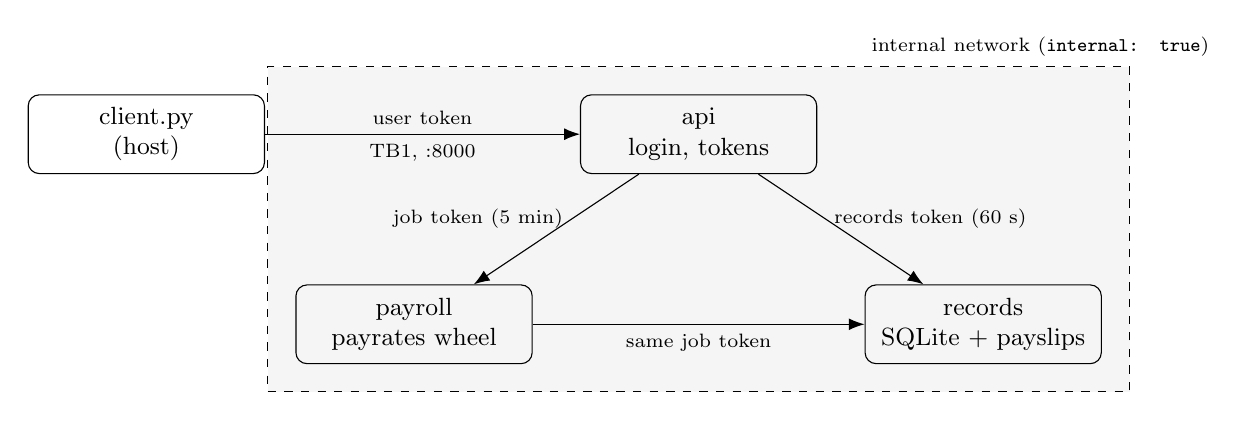
\begin{tikzpicture}[
  box/.style={draw, rounded corners, align=center, minimum width=3cm, minimum height=1cm, font=\small},
  arr/.style={-{Latex[length=2mm]}, font=\scriptsize}]
  \node[box] (client) {client.py\\(host)};
  \node[box, right=4cm of client] (api) {api\\login, tokens};
  \node[box, below right=1.4cm and 0.6cm of api] (records) {records\\SQLite + payslips};
  \node[box, below left=1.4cm and 0.6cm of api] (payroll) {payroll\\payrates wheel};
  \begin{scope}[on background layer]
    \node[draw, dashed, fill=gray!8, inner sep=10pt, fit=(api)(records)(payroll), label={[font=\scriptsize]above right:internal network (\texttt{internal: true})}] {};
  \end{scope}
  \draw[arr] (client) -- node[above]{user token} node[below]{TB1, :8000} (api);
  \draw[arr] (api) -- node[right, pos=0.4]{records token (60 s)} (records);
  \draw[arr] (api) -- node[left, pos=0.4]{job token (5 min)} (payroll);
  \draw[arr] (payroll) -- node[below]{same job token} (records);
\end{tikzpicture}
\caption{Components and the token on each edge. TB1 is the boundary to the host; every service-to-service edge is a boundary that \texttt{records} checks.}
\label{fig:arch}
\end{figure}

\subsection*{Where identity, authority, ownership and dependency trust are established}

\textbf{Identity} is established once, at login. \texttt{records} compares the password with a bcrypt hash (\file{records/app.py:110-115}), and \texttt{api} mints a user token with \texttt{sub}, \texttt{role}, \texttt{aud=api} and a 30-minute expiry (\file{api/app.py:61-65}). After that, the identity is whatever the verified \texttt{sub} claim says. No service reads a user name from the request body or a header.

\textbf{Authority} is the role in the user token plus, for a payslip job, the scope list in the job token. \texttt{api} checks the role before forwarding (for example \file{api/app.py:121} for payslips, \file{:147} for the manager overview). \texttt{records} checks it again.

\textbf{Ownership} is established only in \texttt{records}, because it is the only place that knows who owns a job, an entry or a file. Every query filters on the token's \texttt{sub}: \texttt{WHERE cleaner = ?} for jobs (\file{records/app.py:128-145}), \texttt{own\_job} for clocking (\file{:165}), and the cleaner's own folder for payslips (\file{:235-239}).

\textbf{Dependency trust} is established at build time. The \texttt{payrates} wheel is pinned by SHA-256 in \file{payroll/payrates.txt} and installed by pip in hash-checking mode, without resolving dependencies (\file{payroll/Dockerfile:9}). The pipeline also checks the hash before building. I tested the gate with a wheel that had one extra byte: pip refused it with ``THESE PACKAGES DO NOT MATCH THE HASHES'', expecting \texttt{703d50fb\ldots} and getting \texttt{451130ac\ldots} (\file{evidence/wheel-tamper.log}).

\subsection*{Design principles}

I applied the three principles the assignment names. Each one maps to code and to a test in \file{tests/test_authz.py} that passes on \texttt{v2-fixed} (\file{evidence/v2-fixed/junit.xml}).

\begin{table}[h]
\centering\small
\begin{tabularx}{\textwidth}{@{}lYY@{}}
\toprule
Principle & Implementation & Test \\
\midrule
Least privilege & \texttt{payroll} gets no key, no volume and only the internal network (\file{docker-compose.yml:26-31}). Its job token covers one cleaner, one month, two scopes and 5 minutes (\file{api/app.py:125-131}). & \test{test_payroll_cannot_write_other_month}, \test{test_records_rejects_missing_scope} \\
Complete mediation & Every \texttt{records} route depends on \texttt{claims}, which verifies signature, audience, expiry and required claims (\file{records/app.py:60-68}), whether the caller is \texttt{api} or \texttt{payroll}. & \test{test_records_rejects_expired_job_token}, \test{_wrong_audience}, \test{_token_signed_with_api_key} \\
Fail-safe defaults & A missing header defaults to \texttt{""} and gives 401 (\file{records/app.py:60-63}). An unknown role gives 403 (\file{:71-75}). A token without a \texttt{scope} claim is treated as having none (\file{:91}). & \test{test_no_token_is_rejected}, \test{test_job_token_cannot_use_user_endpoints}, \test{test_cleaner_cannot_call_manager_endpoints} \\
\bottomrule
\end{tabularx}
\caption{Design principles, where they are in the code, and the tests that check them.}
\end{table}

\section{How authority travels through the payslip workflow}

There are three kinds of token, and the difference between them is the main idea of the design. A \emph{user token} (\texttt{aud=api}, 30 min) proves who the client is. For every user request, \texttt{api} mints a \emph{records token} (\texttt{aud=records}, 60 s) with the same \texttt{sub} and \texttt{role}, so \texttt{records} can make its own decision instead of trusting that \texttt{api} already checked (\file{api/app.py:40-44}). For a payslip, \texttt{api} mints a \emph{job token} (\texttt{aud=records}, 5 min) with \texttt{sub}, \texttt{job\_id}, \texttt{month} and \texttt{scope=["entries:read","payslips:write"]} (\file{api/app.py:125-131}).

Together the claims bind the authority to four things the assignment asks for:
\begin{itemize}
  \item \textbf{Service:} \texttt{aud}, and a separate HMAC key per audience. A token signed with the \texttt{api} key is rejected by \texttt{records} (\test{test_records_rejects_token_signed_with_api_key}).
  \item \textbf{Resource:} \texttt{sub} and \texttt{month}.
  \item \textbf{Action:} \texttt{scope} for job tokens, \texttt{role} for records tokens.
  \item \textbf{Validity period:} \texttt{exp}, which PyJWT checks by default.
\end{itemize}

I considered forwarding the user token to \texttt{records} as it is. I did not, for two reasons. First, its audience is \texttt{api}, so accepting it in \texttt{records} would mean a token issued for one service works at another, which is the replay the \texttt{aud} claim exists to stop. Second, it lives for 30 minutes; the records token lives for 60 seconds and exists only for one call. The cost is that \texttt{api} holds the records key, so \texttt{api} is trusted to state the user's identity truthfully. It is not trusted to decide ownership.

A records token has a role and no scope; a job token has a scope and no role. So neither works on the other's endpoints (\file{records/app.py:71}, \file{:90}). I use HS256 because all keys stay inside one compose project; Section~\ref{sec:prod} says what I would change for production.

Figure~\ref{fig:seq} shows the payslip flow and where each check happens.

\begin{figure}[h]
\centering
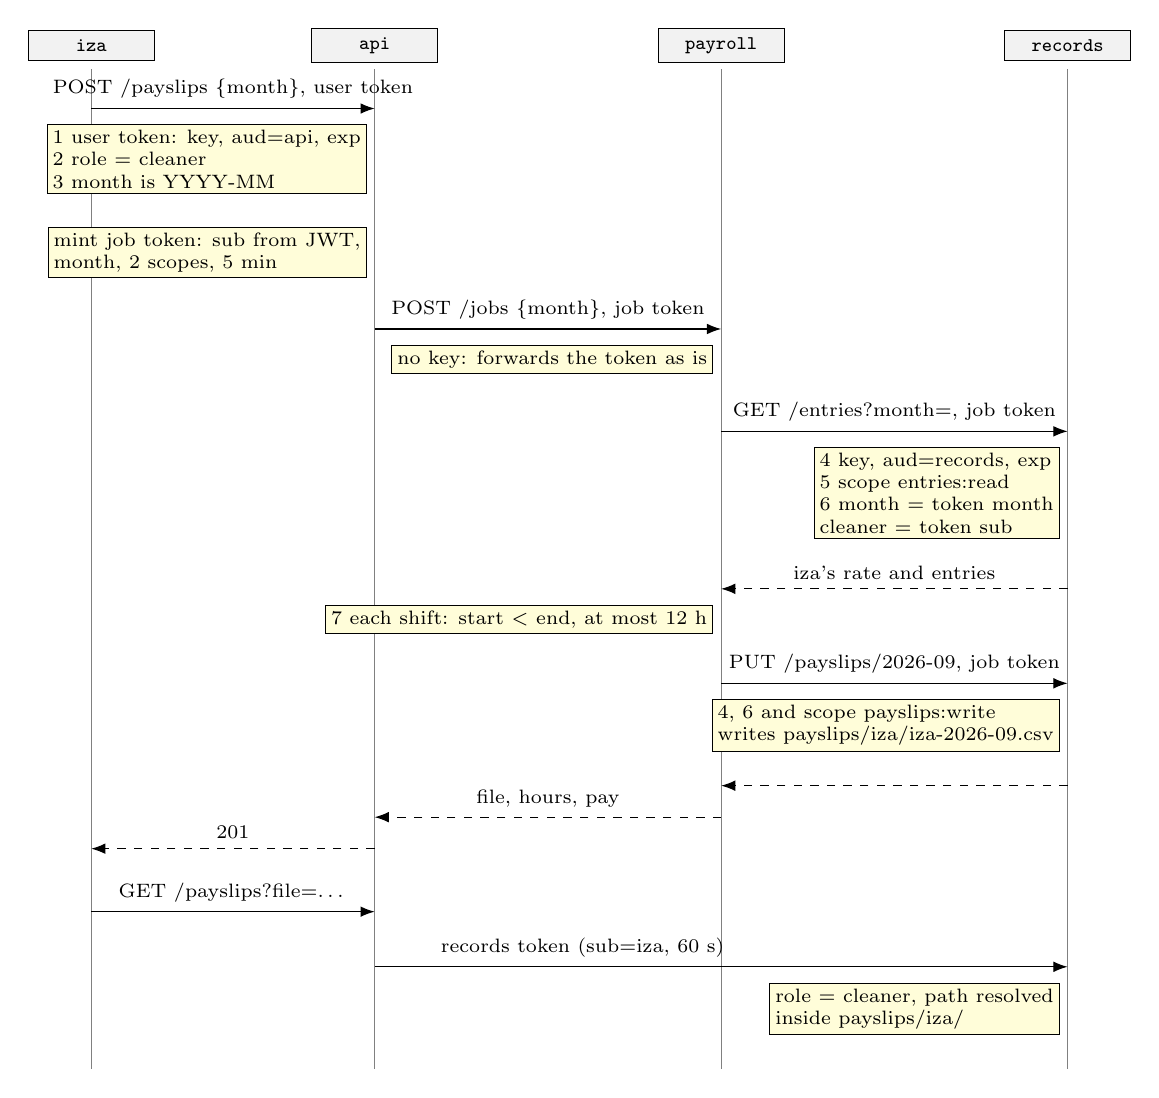
\begin{tikzpicture}[
  font=\scriptsize,
  msg/.style={-{Latex[length=1.8mm]}},
  ret/.style={-{Latex[length=1.8mm]}, dashed},
  chk/.style={draw, fill=yellow!15, align=left, inner sep=2pt, font=\scriptsize}]
  \foreach \x/\n in {0/iza, 3.6/api, 8/payroll, 12.4/records} {
    \node[draw, fill=gray!10, minimum width=1.6cm] at (\x,0) {\texttt{\n}};
    \draw[gray] (\x,-0.3) -- (\x,-13);
  }
  \draw[msg] (0,-0.8) -- node[above]{POST /payslips \{month\}, user token} (3.6,-0.8);
  \node[chk, anchor=north east] at (3.5,-1.0) {1 user token: key, aud=api, exp\\2 role = cleaner\\3 month is YYYY-MM};
  \node[chk, anchor=north east] at (3.5,-2.3) {mint job token: sub from JWT,\\month, 2 scopes, 5 min};
  \draw[msg] (3.6,-3.6) -- node[above]{POST /jobs \{month\}, job token} (8,-3.6);
  \node[chk, anchor=north east] at (7.9,-3.8) {no key: forwards the token as is};
  \draw[msg] (8,-4.9) -- node[above]{GET /entries?month=, job token} (12.4,-4.9);
  \node[chk, anchor=north east] at (12.3,-5.1) {4 key, aud=records, exp\\5 scope entries:read\\6 month = token month\\cleaner = token sub};
  \draw[ret] (12.4,-6.9) -- node[above]{iza's rate and entries} (8,-6.9);
  \node[chk, anchor=north east] at (7.9,-7.1) {7 each shift: start $<$ end, at most 12 h};
  \draw[msg] (8,-8.1) -- node[above]{PUT /payslips/2026-09, job token} (12.4,-8.1);
  \node[chk, anchor=north east] at (12.3,-8.3) {4, 6 and scope payslips:write\\writes payslips/iza/iza-2026-09.csv};
  \draw[ret] (12.4,-9.4) -- (8,-9.4);
  \draw[ret] (8,-9.8) -- node[above]{file, hours, pay} (3.6,-9.8);
  \draw[ret] (3.6,-10.2) -- node[above]{201} (0,-10.2);
  \draw[msg] (0,-11.0) -- node[above]{GET /payslips?file=\ldots} (3.6,-11.0);
  \draw[msg] (3.6,-11.7) -- node[above, pos=0.3]{records token (sub=iza, 60 s)} (12.4,-11.7);
  \node[chk, anchor=north east] at (12.3,-11.9) {role = cleaner, path resolved\\inside payslips/iza/};
\end{tikzpicture}
\caption{Payslip generation and download. The numbered boxes are the checks; \texttt{payroll} cannot change any token it carries.}
\label{fig:seq}
\end{figure}

\subsection*{What stops payroll, a permitted service, from overstepping}

\texttt{payroll} is allowed to read entries and write payslips, so the question is what keeps it inside one job. Four things do.

\begin{enumerate}
  \item \textbf{It cannot change its authority.} It holds no signing key, so it cannot mint a token or edit the one it got. Any change breaks the signature, and \texttt{records} returns 401.
  \item \textbf{The cleaner comes from the token only.} \texttt{records} uses \texttt{who = c["sub"]} and ignores headers and body fields (\file{records/app.py:212}, \file{:224}). \test{test_payroll_cannot_act_for_other_cleaner} sends a valid job token for iza together with \texttt{X-Cleaner-Id: marius}, and gets iza's data and \file{iza-2026-09.csv}.
  \item \textbf{Scope and month are checked on each call} (\file{records/app.py:90-94}). A job token for September cannot write October (\test{test_payroll_cannot_write_other_month}). A token with only \texttt{payslips:write} cannot read entries (\test{test_records_rejects_missing_scope}).
  \item \textbf{The token expires after 5 minutes} (\test{test_records_rejects_expired_job_token}), and the container has nowhere else to send data: \texttt{internal: true} gives it no route out (\file{docker-compose.yml:44}).
\end{enumerate}

\texttt{payroll} also does not trust \texttt{records} completely. Since the CWE-20 fix it rejects any shift that does not end after it starts or that lasts more than 12 hours, before it calculates pay (\file{payroll/app.py:50-52}).

\section{Supply chain}

I did not do the optional supply-chain attack or Experiments A and B. The only supply-chain control is the build-time hash pin from Section~1, and it is tested only by the tampered-wheel run in \file{evidence/wheel-tamper.log}.

\section{How the plan shaped development}

I committed the lifecycle plan (\file{docs/PLAN.md}) in \commit{65be63d}, before any feature code (the first service code is \commit{f6b5d4c}). It fixed the token design, the access-control matrix and the four planned vulnerabilities in advance. That turned out to matter most for the composition bug: the matrix says \texttt{payroll} acts on ``\texttt{sub} and \texttt{month} of token'', so two authorization tests written in Stage~3 (\commit{aa31756}) already encoded that rule before the bug existed.

The plan also decided how I test. Several rules can only be checked by calling \texttt{records} directly, for example that an expired or wrongly scoped job token is rejected, but \texttt{records} has no published port. Instead of opening a port for testing, I run the API tests in a \texttt{tests} container on the internal network (\file{tests/Dockerfile}, run by \texttt{make test}). The tests mint their own job tokens with the records key (\file{tests/conftest.py}) and play the part of \texttt{payroll}. So the authorization tests attack the same interface a compromised \texttt{payroll} would have.

Running the pipeline in a real Jenkins also changed things. Mounting \file{tests/} into the container broke, because Jenkins talks to the host's Docker daemon and the mount path only exists inside the Jenkins container. The tests are now copied into the image (\commit{e2eeee0}). ruff 0.17 also flagged FastAPI's \texttt{Depends()} defaults as B008, so I added an allow-list in \file{ruff.toml} (\commit{ff7cd36}) instead of turning the linter off.

Getting the Jenkins evidence itself took longer than writing the pipeline. I ran Jenkins in a container on my laptop and worked on the project over several days on different Wi-Fi networks. Docker writes a container's DNS server into it when the container starts, so after each network change the Jenkins container still pointed at the old network's DNS server. The first time, the setup wizard could not reach \texttt{updates.jenkins.io} and installed 0 plugins. Later, a branch scan hung because it could not resolve \texttt{api.github.com}, so a push was not built until I restarted the container. One build of \texttt{main} (build 7, on commit \commit{7a0ca4c}) failed with 15 errors because the test container could not resolve \texttt{api} right after a network change; build 8 of the same commit passed all 25 tests (\file{evidence/jenkins/main-build-7/}, \file{main-build-8/}). In the end I ran the Jenkins container in Docker's host network mode, so it uses the laptop's own resolver, which follows network changes. Sadly I also had to reset Jenkins itself several times while developing, which deleted its build history, so the older builds are lost. The runs on both tags in \file{evidence/v1-vulnerable/} and \file{evidence/v2-fixed/} come from a separate Jenkins instance with the same \file{Jenkinsfile}. None of this was a problem in the application, but it shows that CI results are only as reliable as the machine they run on, and a shared build server would avoid it.

When I planted V4 in \commit{baed1bb}, those two tests failed: \test{test_payroll_cannot_act_for_other_cleaner} and \test{test_api_ignores_cleaner_in_payslip_request}. That failure, not static analysis, is what blocked the vulnerable build. The gate decisions were:

\begin{table}[h]
\centering\small
\begin{tabularx}{\textwidth}{@{}lYl@{}}
\toprule
Gate & Result & Evidence \\
\midrule
Requirements & Plan reviewed before code; roles and architecture unchanged afterwards & \commit{65be63d} \\
Build & Wheel hash OK; tampered wheel refused & \file{evidence/v2-fixed/pipeline.log}, \file{wheel-tamper.log} \\
Testing, \texttt{v1-vulnerable} & Blocked: 2 failed, 23 passed, ``Finished: FAILURE'' & \file{evidence/v1-vulnerable/pipeline.log} \\
Testing, \texttt{v2-fixed} & Passed: 25 + 3 tests, no bandit HIGH, 0 vulnerabilities in 24 audited packages & \file{evidence/v2-fixed/pipeline.log} \\
\bottomrule
\end{tabularx}
\caption{Gate decisions from the Jenkins runs on both tags.}
\end{table}

Two results did not match the plan. First, the blocking rule ``any bandit HIGH'' did not catch the SQL injection. Bandit reported it as B608 with MEDIUM severity and LOW confidence at \file{records/app.py:143} (\file{evidence/v1-vulnerable/bandit.json}). I kept the rule and recorded the gap instead of lowering the threshold after seeing the result. Second, the path traversal and SQL injection were not caught by any Stage~3 test, because those tests did not try \texttt{../} or quote characters. Only the exploit tests show them. A test suite checks the rules I thought to write down, not every input.

\subsection*{Where each protection comes from}

\begin{itemize}
  \item \textbf{Language and runtime.} Python has no manual memory management, so the memory-safety weaknesses in the catalog (CWE-787, CWE-416) do not apply. \texttt{pathlib}'s \texttt{resolve()} and \texttt{is\_relative\_to()} do the canonicalisation for the CWE-22 fix. \texttt{sqlite3} placeholders keep data out of SQL syntax, and \texttt{execute} runs only one statement, so stacked queries fail even in the vulnerable version.
  \item \textbf{Libraries.} PyJWT checks signature, \texttt{exp} and \texttt{aud}, and the \texttt{require} option rejects tokens with missing claims. bcrypt handles password hashing. Pydantic rejects request bodies with the wrong types, for example a clock time that is not a datetime. Pydantic only checks syntax, not meaning, which is why CWE-20 was still possible.
  \item \textbf{Application logic.} Role, ownership, scope and month checks in \texttt{records}; role checks repeated in \texttt{api}; shift validation in both \texttt{records} and \texttt{payroll}.
  \item \textbf{Deployment configuration.} Only \texttt{api} is published. \texttt{records} and \texttt{payroll} sit on an \texttt{internal: true} network. Every container runs as a non-root user (\texttt{USER app} in each Dockerfile). \texttt{payroll} has no volume, and the wheel is installed by hash.
\end{itemize}

\subsection*{What a production release would need}
\label{sec:prod}

This is a coursework deployment, and several things are deliberately simple.

\begin{itemize}
  \item \textbf{Secrets management.} The JWT keys have development defaults in \file{docker-compose.yml:12-13}. In production they would come from a secret store (for example Docker secrets or Vault) and never appear in the repository.
  \item \textbf{TLS between services.} All traffic is plain HTTP, including bearer tokens on the internal network. I would use TLS at the edge and mutual TLS between services, so that \texttt{records} also knows which service is calling and not only which token it carries.
  \item \textbf{Key rotation.} One static key per audience means a leaked \texttt{RECORDS\_JWT\_KEY} lets anyone mint job tokens for any cleaner. I would switch to asymmetric keys (ES256): \texttt{api} signs, \texttt{records} verifies with a public key published with a \texttt{kid}, so keys can rotate without redeploying \texttt{records}.
  \item \textbf{Logging and monitoring.} There is no audit log. I would log every authorization decision in \texttt{records} (who, what, allowed or denied) and alert on repeated 403s. Repudiation is currently covered only by storing the creator's \texttt{sub} on each entry.
  \item \textbf{Signed artifacts.} The wheel hash proves the bytes did not change after I approved them, not who built them. I would sign the wheel and the container images (for example with Sigstore) and verify the signatures at deploy time.
\end{itemize}

Rate limiting on login and the internal \texttt{/login} endpoint, which any container on the network can call, would also need attention.

\section{Planted vulnerabilities}

I planted four vulnerabilities, each in its own commit with a \texttt{\# VULN} comment, and showed each one with a test in \file{tests/exploits/}. Tag \texttt{v1-vulnerable} (\commit{305067f}) contains all four, and \texttt{v2-fixed} (\commit{9661bad}) contains all the fixes. The full analysis, in the catalog's six sections, is in \file{docs/VULNERABILITIES.md}.

\begin{table}[h]
\centering\small
\begin{tabularx}{\textwidth}{@{}lYll@{}}
\toprule
CWE & What happened & Planted & Fixed \\
\midrule
CWE-22 & The payslip file name was joined onto the cleaner's folder without canonicalisation; iza downloaded \texttt{../marius/marius-2026-09.csv} & \commit{405b6f1} & \commit{4853573} \\
CWE-89 & The cleaner's job search built SQL with an f-string; a search text that closes the quote and appends \texttt{OR 1=1} and an SQL comment returned every job & \commit{9ef01b7} & \commit{00f06ef} \\
CWE-20 & Clock-out accepted any end time and \texttt{payroll} paid it; a 30-hour shift added exactly 30 hours to iza's payslip & \commit{c929555} & \commit{552b4d8} \\
CWE-862 (composition) & \texttt{api} took \texttt{cleaner\_id} from the body, \texttt{payroll} sent it as \texttt{X-Cleaner-Id}, \texttt{records} trusted it; iza got marius's payslip with his 210 DKK rate & \commit{baed1bb} & \commit{9661bad} \\
\bottomrule
\end{tabularx}
\caption{Planted vulnerabilities with the commits that added and removed them.}
\end{table}

The composition bug is the one I learned most from. Seen alone, each service looks correct: \texttt{api} authenticates, \texttt{payroll} forwards, and \texttt{records} verifies the job token completely. The bug only exists because the cleaner crossed the services in a plain field next to the token, and \texttt{records} treated being on the internal network as being trusted. The fix removes that field and binds the cleaner to the signed \texttt{sub} only. My takeaway is that every piece of authority has to travel inside something the receiver can verify; anything next to the token is just input.

The other three taught smaller lessons. The CWE-22 fix shows that choosing the folder from the token is not enough when the file name can still leave it; the check has to be on the final, resolved path. Exploiting it also needed a precondition I did not expect: Linux only resolves \texttt{iza/..} if \file{payslips/iza/} exists, so iza first had to generate her own payslip. The CWE-89 case was the only one that static analysis noticed at all. The CWE-20 fix is the only one where I added a check in a second service: \texttt{records} validates at the point of entry, and \texttt{payroll} validates again before paying, because the catalog names ``assuming another component has already validated the input'' as the underlying factor. No test reaches the \texttt{payroll} check alone, since \texttt{records} now rejects bad shifts first; I state that gap in \file{docs/VULNERABILITIES.md}.

\appendix
\section{Evidence index}

\begin{table}[h]
\centering\small
\begin{tabularx}{\textwidth}{@{}lY@{}}
\toprule
Item & Location \\
\midrule
Requirements, plan, decisions & \file{docs/REQUIREMENTS.md} (\commit{4190cdf}), \file{docs/PLAN.md} (\commit{65be63d}), \file{docs/DECISIONS.md} \\
Architecture, threat model, access control & \file{docs/ARCHITECTURE.md}, \file{docs/THREAT_MODEL.md}, \file{docs/ACCESS_CONTROL.md} \\
Pipeline definition & \file{Jenkinsfile} (\commit{305067f}), \file{jenkins/Dockerfile} \\
Pipeline runs & \file{evidence/v1-vulnerable/}, \file{evidence/v2-fixed/} (console log, \file{bandit.json}, \file{pip-audit.json}, \file{junit.xml}) \\
Hash gate & \file{evidence/wheel-tamper.log} \\
Tests & \file{tests/test_functional.py} (7), \file{tests/test_authz.py} (13), \file{tests/exploits/} (4), \file{payrates/tests/} (3) \\
\bottomrule
\end{tabularx}
\end{table}

\end{document}
